\documentclass{article}
\usepackage{amsmath}
\usepackage[table]{xcolor}
\usepackage{array}
\usepackage{graphicx}
\usepackage{enumitem}
\usepackage{etoolbox}

\usepackage[utf8]{inputenc}
\usepackage[ngerman]{babel}
\usepackage{anysize}
\usepackage{amssymb}
\usepackage{amsmath}
\usepackage{eqnarray}
\newtheorem{mydef}{Definition}
\newtheorem{alg}{Algorithmus}
\usepackage{lmodern}
\usepackage{url}
\usepackage{setspace}
\usepackage{chemformula}
\usepackage{multicol,multirow,caption}
\usepackage{fmtcount} 
\usepackage{gensymb}
\usepackage{wrapfig}
\usepackage{float}
\usepackage{tabularx}
\marginsize{10mm}{10mm}{5mm}{5mm} % l|r|o|u
\newcommand{\diff}{\mathop{} \mathrm{d}}
\newcommand{\del}{\mathop{} \partial}
\usepackage[headsepline]{scrlayer-scrpage}
\setlength{\headsep}{0.05cm}



\clearpairofpagestyles
\ihead{Cedric Renda }
\chead{Physik 2}
\ohead{FS21: \today}
%\setkomafont{pageheadfoot}{\sffamily}
\usepackage{lastpage}


\title{Physik 2}
\author{Cedric Renda}
\date{\today}

\AtBeginEnvironment{tabular}{%
	\setlist[itemize]{
		nosep,
		topsep     = 0pt,
		partopsep  = 0pt,
		leftmargin = *,
		label      = $\bullet$,
		before     = \vspace{-0.6\baselineskip},
		after      = \vspace{-\baselineskip}
	}%
}

\newcommand{\rotcell}[1]{%
	\rotatebox[origin=c]{90}{\begin{tabular}{c}#1\end{tabular}}%
}
\newcolumntype{L}[1]{>{\raggedright\arraybackslash}m{#1}}
\newcolumntype{C}[1]{>{\centering\arraybackslash}m{#1}}
\newcolumntype{R}[1]{>{\raggedleft\arraybackslash}m{#1}}
\newcolumntype{N}{@{}m{0pt}@{}}
%\renewcommand{\arraystretch}{3}
\begin{document}
	\centering
	%\begin{center}
	%
\title{Inhaltsverzeichnis}
\begin{tabular}{L{5cm} c}
	Konstanten & 1\\
	Geometrie & 1\\
	Allgemeines & 1\\
	Wellen&2\\
\end{tabular}
\newpage
	%Mathe 
%	\ofoot{Seite \thepage \hspace{1pt} von \pageref{LastPage}}
	\setcounter{page}{1}
	%\setlength{\columnseprule}{0.4pt}
	%
		\begin{tabular}{ | c   p{18cm} |}
			\hline
			%\rowcolor{blue!30}
			\cellcolor{black}\rotcell{\large\textbf{\textcolor{white}{Konstanten}}}  &
			\setlength{\extrarowheight}{5pt}			
			\begin{tabular}{L{5cm} L{8cm} L{3.8cm}}
				\textbf{Elektrische Feldkonstante}
				Permittivität von Vakuum &$\varepsilon_{0}=8.854 \times 10^{-12} \mathrm{~F} / \mathrm{m} $&$\left[\varepsilon_{0}\right]=\frac{\mathrm{F}}{\mathrm{m}}=\frac{\mathrm{As}}{\mathrm{Vm}}=\frac{\mathrm{C}^{2}}{\mathrm{Nm}^{2}}$\\[5pt]
				
				
			\rowcolor[rgb]{0.91,0.91,0.91}
			\textbf{Lichtgeschwindigkeit} &$\displaystyle c_0=2.99792 \times 10^{8} \mathrm{m}/\mathrm{s}=\frac{1}{\sqrt{\varepsilon_{0} \mu_{0}}}=\frac{E_{0}}{B_{0}} $
			&$\left[c_{0}\right]=\frac{\mathrm{m}}{\mathrm{s}}$\\[5pt]
				
				
			\rowcolor[rgb]{1,1,1}\textbf{Magnetische Feldkonstante}
				Permeabilität von Vakuum 
				&$\mu_{0}=4 \pi \times 10^{-7} \mathrm{H} / \mathrm{m} $&$\left[\mu_{0}\right]=\frac{\mathrm{H}}{\mathrm{m}}=\frac{\mathrm{V} \mathrm{s}}{\mathrm{A} \mathrm{m}}=\frac{\mathrm{Tm}}{\mathrm{A}}$\\[10pt]
				
			\rowcolor[rgb]{0.91,0.91,0.91}
			\textbf{Masse des Elektrons} (Ruhemasse, $v<<c_0$)
			&$m_{e}=9.109 \times 10^{-31} \mathrm{~kg} $&$\left[m_{e}\right]=\mathrm{kg}$\\[5pt]
			
				
		\rowcolor[rgb]{1,1,1}\textbf{Elementarladung}
		(Ladung des Elektrons $q_e = -e$)
		&$e=1.602 \times 10^{-19} \mathrm{C} $&$[e]=\mathrm{As}=\mathrm{C}$\\[5pt]
	
			\end{tabular}\\
			\hline
		\end{tabular}

	\begin{tabular}{c}
	
	\begin{tabular}{ | c   p{18cm} |}
		\hline
		%\rowcolor{blue!30}
		\cellcolor{black}\rotcell{\large\textbf{\textcolor{white}{Konstanten}}}  &
		\setlength{\extrarowheight}{5pt}			
		\begin{tabular}{L{5cm} L{8cm} L{3.8cm}}
			\textbf{Elektrische Feldkonstante}
			Permittivität von Vakuum &$\varepsilon_{0}=8.854 \times 10^{-12} \mathrm{~F} / \mathrm{m} $&$\left[\varepsilon_{0}\right]=\frac{\mathrm{F}}{\mathrm{m}}=\frac{\mathrm{As}}{\mathrm{Vm}}=\frac{\mathrm{C}^{2}}{\mathrm{Nm}^{2}}$\\[5pt]
			
			
			\rowcolor[rgb]{0.91,0.91,0.91}
			\textbf{Lichtgeschwindigkeit} &$\displaystyle c_0=2.99792 \times 10^{8} \mathrm{m}/\mathrm{s}=\frac{1}{\sqrt{\varepsilon_{0} \mu_{0}}}=\frac{E_{0}}{B_{0}} $
			&$\left[c_{0}\right]=\frac{\mathrm{m}}{\mathrm{s}}$\\[5pt]
			
			
			\rowcolor[rgb]{1,1,1}\textbf{Magnetische Feldkonstante}
			Permeabilität von Vakuum 
			&$\mu_{0}=4 \pi \times 10^{-7} \mathrm{H} / \mathrm{m} $&$\left[\mu_{0}\right]=\frac{\mathrm{H}}{\mathrm{m}}=\frac{\mathrm{V} \mathrm{s}}{\mathrm{A} \mathrm{m}}=\frac{\mathrm{Tm}}{\mathrm{A}}$\\[10pt]
			
			\rowcolor[rgb]{0.91,0.91,0.91}
			\textbf{Masse des Elektrons} (Ruhemasse, $v<<c_0$)
			&$m_{e}=9.109 \times 10^{-31} \mathrm{~kg} $&$\left[m_{e}\right]=\mathrm{kg}$\\[5pt]
			
			
			\rowcolor[rgb]{1,1,1}\textbf{Elementarladung}
			(Ladung des Elektrons $q_e = -e$)
			&$e=1.602 \times 10^{-19} \mathrm{C} $&$[e]=\mathrm{As}=\mathrm{C}$\\[5pt]
			
		\end{tabular}\\
		\hline
	\end{tabular}\\
\begin{tabular}{ | c   p{18cm} |}
	\hline
	\cellcolor{black}\rotcell{\large\textbf{\textcolor{white}{Geometrie}}}  &
	\begin{tabular}{p{18cm}}	
		\setlength{\extrarowheight}{10pt}			
		\begin{tabular}{L{5.6cm}| L{5.6cm}| L{5.8cm}}
			\multirow{2}{*}{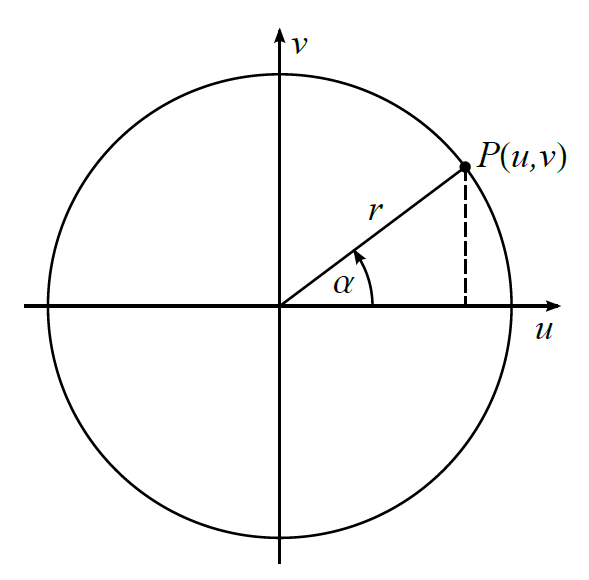
\includegraphics[width=5.6cm]{kreis.png}}
			& $\displaystyle \sin(\alpha)=\frac{v}{r}$ \qquad  $\displaystyle\cos(\alpha)=\frac{u}{r}$ &  $\displaystyle\sin(\alpha)^2  + \cos(\alpha)^2=1$\\
			&  $\displaystyle \tan(\alpha)=\frac{\sin(\alpha)}{\cos(\alpha)}$&$\displaystyle \cot(\alpha)=\frac{\cos(\alpha)}{\sin(\alpha)}$\\
			
			&$\displaystyle \sin(\alpha)=\sin(\alpha+ 2\pi)$ & $\cos(\alpha)= \cos( 2\pi-\alpha)$\\
			
			&$\displaystyle -\sin(\alpha)=\sin(-\alpha)$ & $\cos(-\alpha)= \cos(\alpha)$\\
			
			&$\displaystyle \tan(\alpha)=\tan(\alpha+ \pi)$ & $\tan(-\alpha)= -\tan(\alpha)$\\
			
			&$\displaystyle \sin(\alpha\pm\beta)=\sin(\alpha)\cos(\beta)\pm\cos(\alpha)\sin(\beta)$ & $\sin(2\alpha)= 2\sin(\alpha)\cos(\alpha)$\\
			
			&$\displaystyle \cos(\alpha\pm\beta)=\cos(\alpha)\cos(\beta)\mp\sin(\alpha)\sin(\beta)$ & $\cos(2\alpha)= \cos^2(\alpha)-\sin^2(\alpha)$\\
			
			&$\displaystyle \cos(\arcsin(x))=\sin(\arccos(x))= \sqrt{1-x^2}$ & $\cos(2\alpha)= 2\cos^2(\alpha)-1$\\
			
			
			\textbf{Kartesische Koordinaten}& \textbf{Zylindrische Koordinaten} & \textbf{Sphärische Koordinaten}\\
			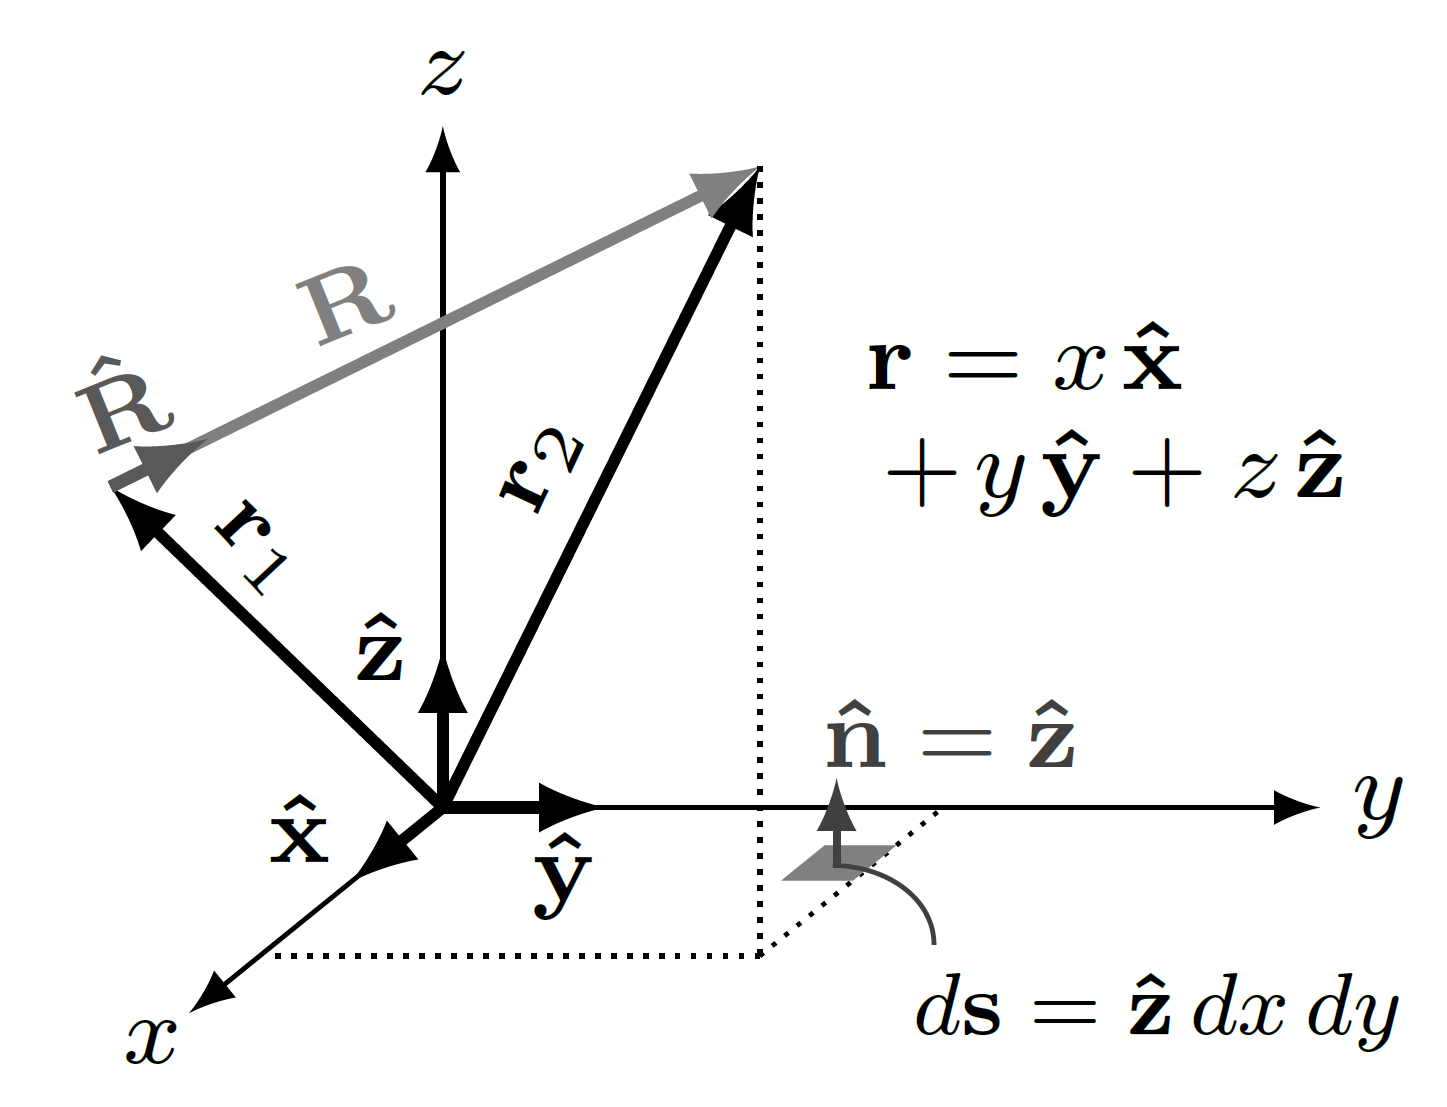
\includegraphics[width=5.6cm]{kartesische.png}& 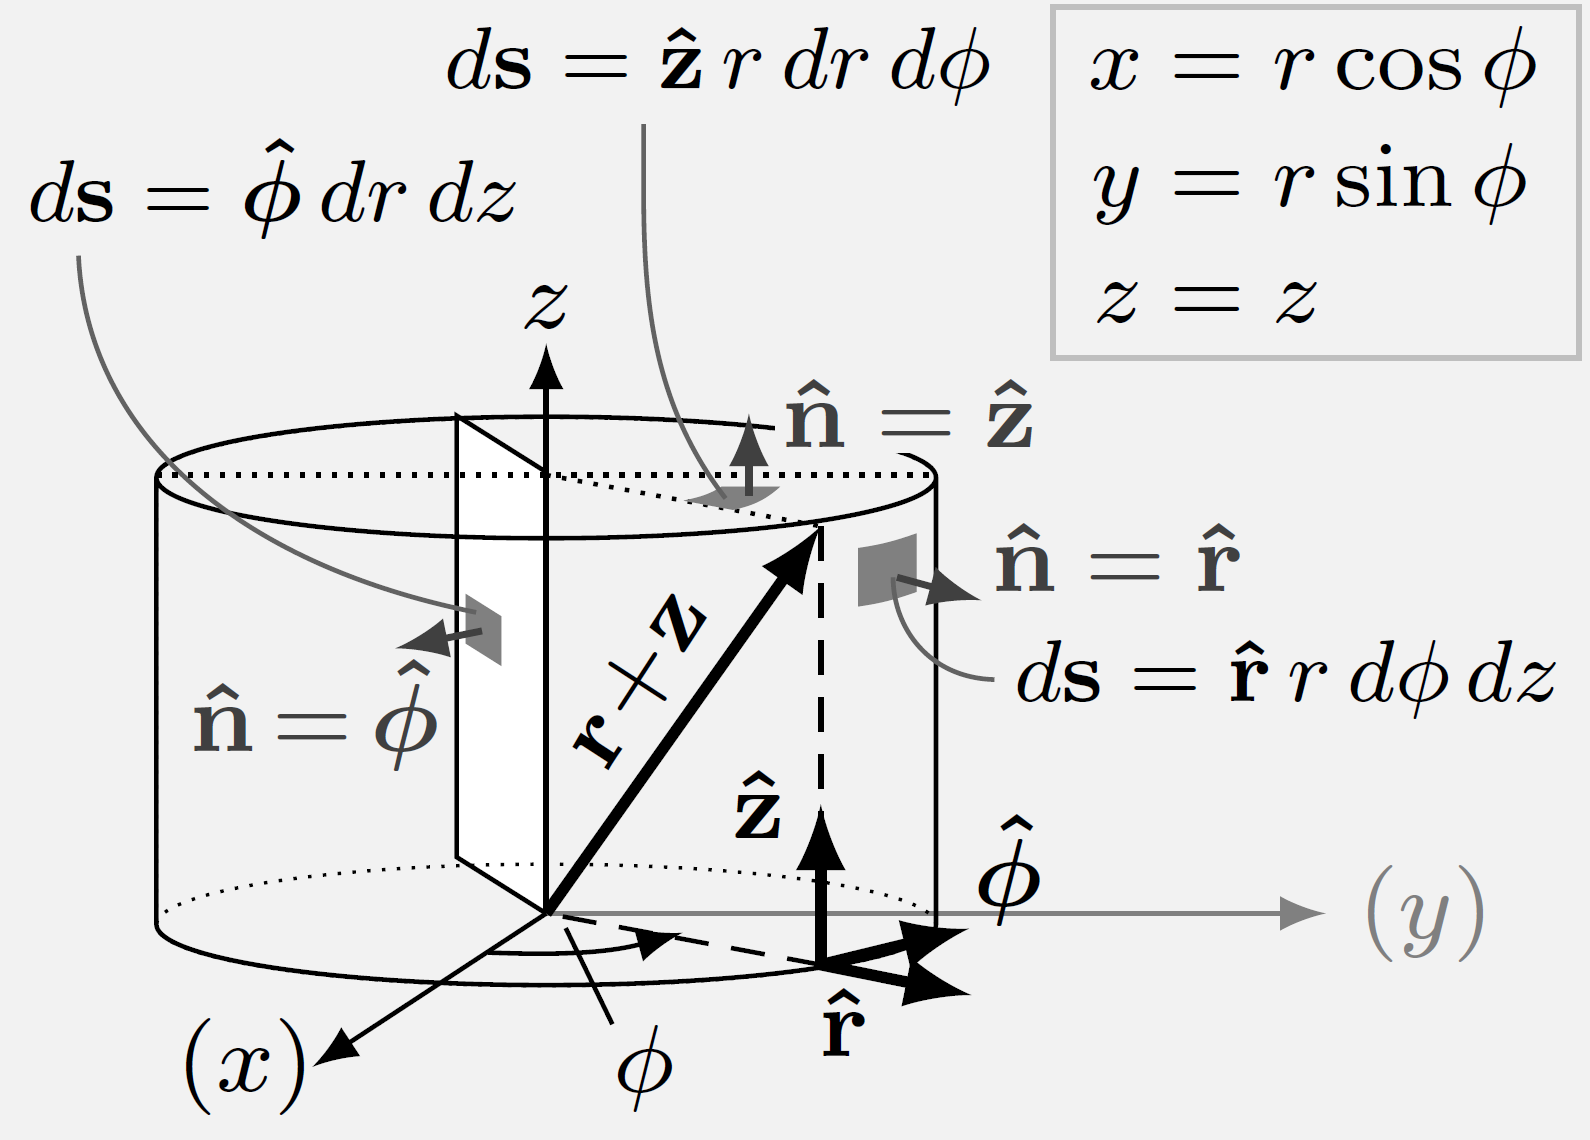
\includegraphics[width=5.6cm]{zylindrische.png}& 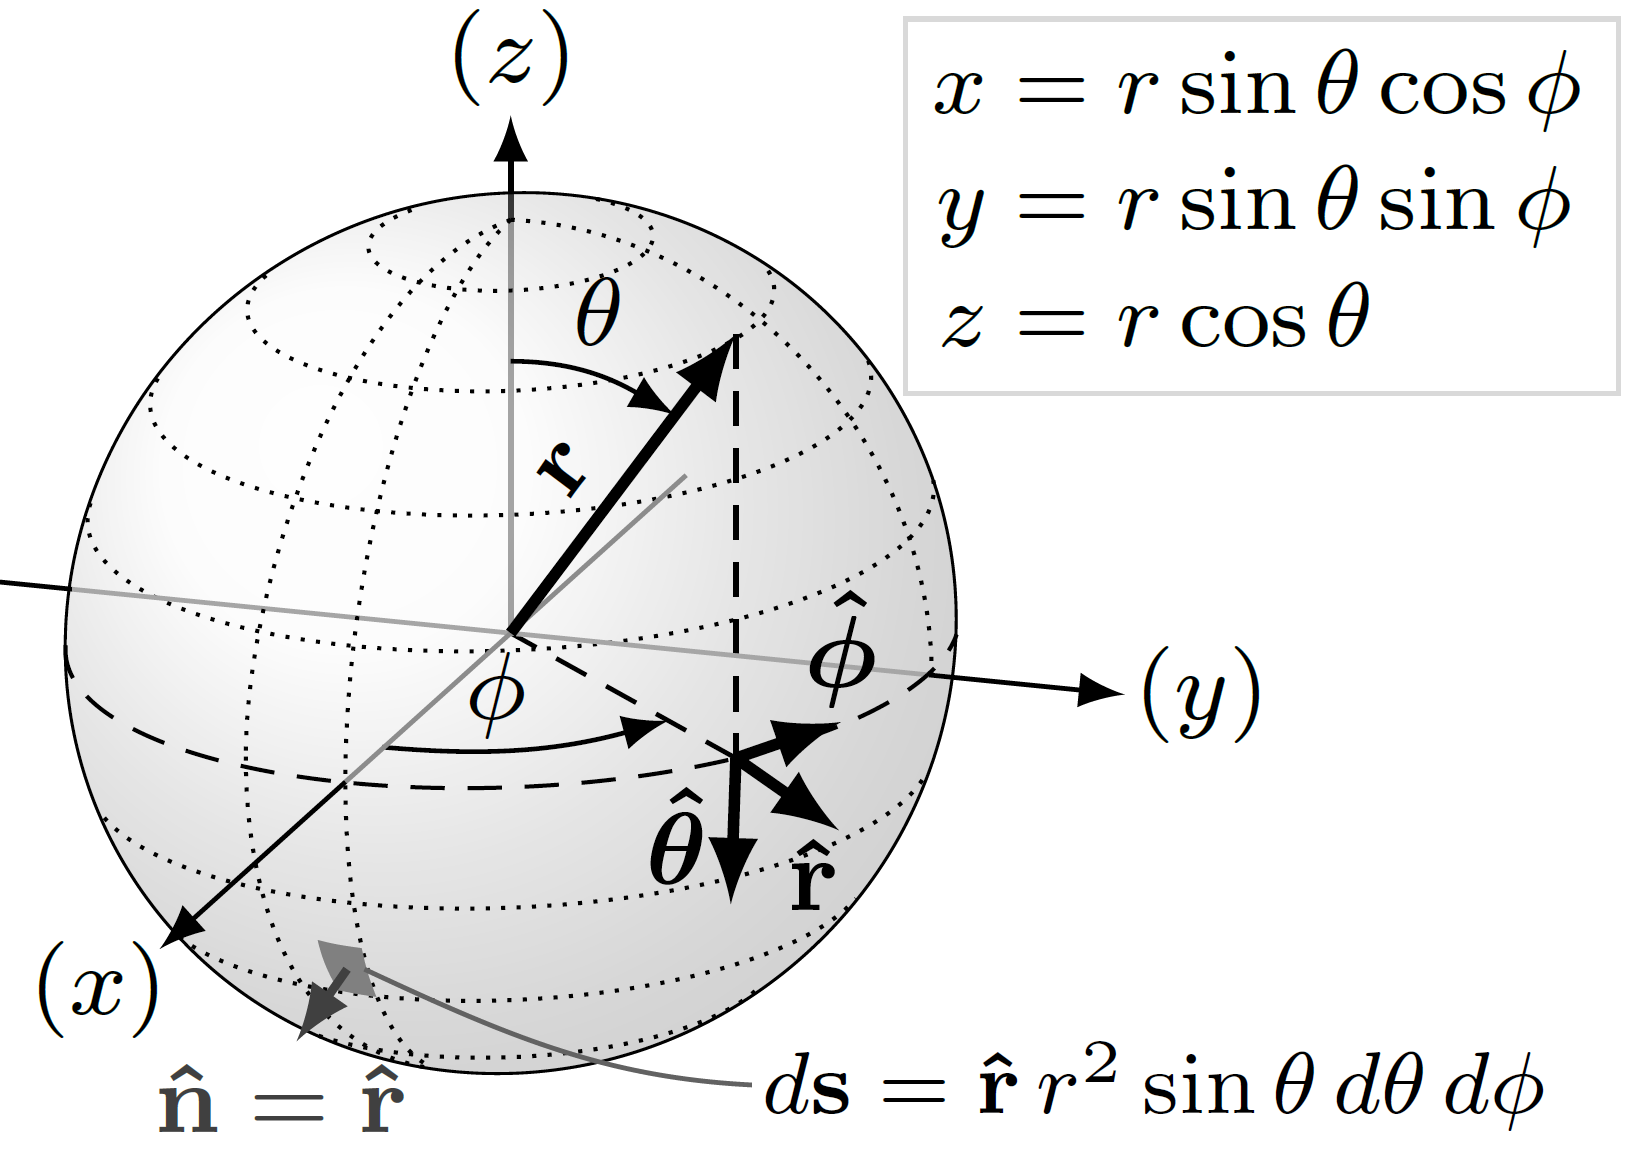
\includegraphics[width=5.6cm]{spherische.png}\\
			Volumenelement: $ d v=d x d y d z$&Volumenelement: $d v = r d r d \phi d z$&Volumenelement: $d v=r^{2} \sin \theta d r d \theta d \phi$\\
			\textbf{Kreis} Umfang $U=2\pi r$&\textbf{Oberfläche} $A=2\pi rh+2\pi r^2$ & \textbf{Oberfläche} $A=4\pi r^2$ \\
			\textbf{Kreis} Fläche $U=2\pi r^2$&\textbf{Volumen} $V=\pi r^2h$ & \textbf{Volumen} $V=\frac{4}{3}\pi r^3$ \\
			
			
			
		\end{tabular}\\
		%\setlength{\extrarowheight}{5pt}
		\begin{tabular}{L{5cm} L{7.8cm} L{3.8cm}}
			\rowcolor[rgb]{0.91,0.91,0.91}\textbf{Vektorprodukt}  $\mathbb{R}^3 \times \mathbb{R}^3 \rightarrow \mathbb{R}^3$&
			$\left(\begin{array}{c}a_{x} \\ a_{y} \\ a_{z}\end{array}\right) \times\left(\begin{array}{l}b_{x} \\ b_{y} \\ b_{z}\end{array}\right)=\left(\begin{array}{c}a_{y} b_{z}-a_{z} b_{y} \\ a_{z} b_{x}-a_{x} b_{z} \\ a_{x} b_{y}-a_{y} b_{x}\end{array}\right) $&
			$ \vec{a} \times \vec{b}=-(\vec{b} \times \vec{a})$	 \\[10pt]
			
			\rowcolor[rgb]{1,1,1}\textbf{Skalarprodukt}  $\mathbb{R}^3 \times \mathbb{R}^3 \rightarrow \mathbb{R}$&
			$\left(\begin{array}{l}a_{x} \\ a_{y} \\ a_{z}\end{array}\right) \cdot\left(\begin{array}{l}b_{x} \\ b_{y} \\ b_{z}\end{array}\right)=a_{x} b_{x}+a_{y} b_{y}+a_{z} b_{z}=\vec{a} \cdot \vec{b} $&
			$\displaystyle \cos (\varphi)=\frac{\vec{a} \cdot \vec{b}}{|\vec{a}| \cdot|\vec{b}|}$\\[5pt]
			
			\rowcolor[rgb]{0.91,0.91,0.91}
			\textbf{Komplexe Polarform}
			&$\displaystyle z = r\cdot e^{i\varphi} = r\cos(\varphi)+i\sin(\varphi)$
			&$\displaystyle z = a +bi$\qquad $r= |z|= \sqrt{a^2 +b^2}$ \\[5pt]
			
			\rowcolor[rgb]{1,1,1}
			\textbf {Komplexe Winkel} &$\displaystyle \varphi= \arg(z)= \begin{cases}\displaystyle \arccos(\frac{a}{r})  \\ \displaystyle -\arccos(\frac{a}{r} ) \end{cases} $&
			$\displaystyle \begin{cases} b\geq0 \\ \displaystyle b<0 \end{cases}$\\[5pt]
			
			\rowcolor[rgb]{0.91,0.91,0.91}\textbf{Arithmetik}&
			$z_1 = r_1 cis(\varphi_1)= r_1e^{i\varphi_1}$&
			$z_2 = r_2 cis(\varphi_2)= r_2e^{i\varphi_2}$		\\
			
			\textbf{Winkel Addieren}&$z_1\cdot z_2 = r_1\cdot r_2 \text{cis}(\varphi_1+\varphi_2)$&	\\
			
			\textbf{Winkel Subtrahieren}&$z_1/ z_2 = r_1/r_2 cis(\varphi_1-\varphi_2)$&	\\[5pt]
			
			
			
			
			
		\end{tabular}\\[5pt]
	\end{tabular}\\
	\hline	
\end{tabular}

	
\end{tabular}
	

	%
		\begin{tabular}{ | c   p{18cm} |}
			\hline
			%\rowcolor{blue!30}
			\cellcolor{black}\rotcell{\large\textbf{\textcolor{white}{Allgemein}}}  &
			\setlength{\extrarowheight}{5pt}			
			\begin{tabular}{L{5cm} L{6.5cm} L{5.3cm}}
				\textbf{Arbeit, Energie}
				 &$\Delta W=\int_{L} \mathbf{F} \cdot d \mathbf{l}=W_{1}-W_{2}$
				&$[\Delta W]=[W]=\mathrm{J}=\mathrm{W} \mathrm{s}$, \qquad $[F]=\mathrm{N}=\mathrm{kg} \cdot \mathrm{m} / \mathrm{s}^{2}$ \\[5pt]
				
				
			\rowcolor[rgb]{0.91,0.91,0.91}
			\textbf{Drehmoment} &
			$\mathbf{T}=\mathbf{r} \times \mathbf{F} \quad$ (T auf Drehachse)&
			$[T]=\mathrm{Nm}=\mathrm{kg} \cdot \mathrm{m}^2 / \mathrm{s}^{2},[r]=\mathrm{m}$\\[5pt]
				
				
			\rowcolor[rgb]{1,1,1}\textbf{Zentripedalkraft}&
			$\mathbf{F}=\frac{m v^{2}}{r}(-\hat{\mathbf{r}})=-m \omega^{2} \mathbf{r}$&
			$[m]=\mathrm{kg},[r]=\mathrm{m}$, \qquad	$[v]=m / s,[\omega]=\mathrm{rad} / s$		\\[10pt]
				
			\rowcolor[rgb]{0.91,0.91,0.91}
			\textbf{Lorenzkraft} &$\mathbf{F}_{L}=\mathbf{F}_{C}+\mathbf{F}_{A}=q(\mathbf{E}+\mathbf{v} \times \mathbf{B})$&
			$[E]=\mathrm{V} / \mathrm{m},[B]=\mathrm{A} / \mathrm{m}$   
			\qquad $[v]=\mathrm{m} / \mathrm{s},[l]=\mathrm{m}$ \\[5pt]
			
				
			\rowcolor[rgb]{1,1,1}\textbf{Drehimpuls}&
			$\boldsymbol{L}=\boldsymbol{r} \times \boldsymbol{p}$&
			$[L]=\mathrm{kg} \cdot \mathrm{m}^2 / \mathrm{s}$\\[5pt]
			
			\rowcolor[rgb]{0.91,0.91,0.91}\textbf{Drallsatz}&$M=\dot{L}$ &\\
			
	
			\end{tabular}\\
			\hline
		\end{tabular}

	
	% Wellen Schwingungen
	
		\begin{tabular}{ | c   p{18cm} |}
			\hline
			\cellcolor{black}\rotcell{\large\textbf{\textcolor{white}{Wellen}}}  &
			\setlength{\extrarowheight}{10pt}			
			\begin{tabular}{L{5cm} L{7cm} L{5cm}}
				\textbf{Wellengleichung}
				 1 und 3 Dimensional &
				 $\displaystyle \frac{\partial^{2} \xi}{\partial t^{2}}-v^{2} \frac{\partial^{2} \xi}{\partial x^{2}}=0$ \qquad $\displaystyle\frac{\partial^{2} \vec{\xi}}{\partial t^{2}}-v^{2} \Delta \vec{\xi}=0$ &Allg. Lösung $\xi(x, t)=f(x \pm v t)$ \\[10pt]
				
				\rowcolor[rgb]{0.91,0.91,0.91}
				Harmonische Lösung: & 
				$\displaystyle \xi(x, t) =\xi_{0} \sin (k(x \pm v t))=\xi_{0} \sin (k x \pm \omega t) =\xi_{0} e^{i(k x \pm \omega t)}
				$ & 
				$-v$ rechtslaufend $+v$ linkslaufend \\[10pt]
				
				\rowcolor[rgb]{1,1,1}
				\textbf{Wellenlänge \& Wellenzahl}  &$\displaystyle \lambda=\frac{v}{f}=\frac{2\pi}{k}=v\cdot T$\qquad $\displaystyle k=|\mathbf{k}|=\omega \sqrt{\varepsilon \mu}=\frac{\omega}{v}=\frac{2 \pi}{\lambda}$ & $\left[\lambda\right]=\mathrm{m}$ $[k]=\mathrm{rad} / \mathrm{m}$\\[10pt]
				
				\rowcolor[rgb]{0.91,0.91,0.91}
				\textbf{Seilwelle} Transversal (Zugspannung $\mathrm{S}$) & $\displaystyle v^{2}=\frac{S}{\rho} \quad$ , $\displaystyle\quad S=\frac{F}{A\quad}$ , $\displaystyle \quad\rho=\frac{m}{V} \quad$&
				$\left[\mathrm{F}\right]=\mathrm{kg}\cdot\mathrm{m}/\mathrm{s} ^{2}$\qquad\qquad\qquad
				Dichte
				$\left[\mathrm{\rho}\right]=\mathrm{kg}/\mathrm{m}^{3}$ \\[5pt]
				
				
				\rowcolor[rgb]{1,1,1}
				\textbf{Festkörper} Longitudalwelle \quad ($E$ Elastizitätmodul)  & $\displaystyle v^{2}=\frac{E}{\rho} \quad$ , $\displaystyle\quad E=\sigma\frac{l}{\Delta l}$&
				$\left[\mathrm{E}\right]=\mathrm{N}/\mathrm{m}^{-2}$\qquad
				Normalspannung
				 $\left[\mathrm{\sigma}\right]=\frac{\mathrm{dF_{\bot}}}{da}\mathrm{N}/\mathrm{m}^{-2}$ \\[5pt]
				
				
				\rowcolor[rgb]{0.91,0.91,0.91}
				\textbf{Ebene Welle}  \qquad \qquad harmonische Welle  & $\displaystyle \vec{\xi}(x, y, z, t)=\vec{A} e^{i(\vec{k} \cdot \vec{r}-\omega t)}$&
				(Die zu $\vec{k}$ senkrechte Ebene ist $\vec{k} \cdot \vec{r}=$ konst. $)$\\[5pt]
				
				\rowcolor[rgb]{1,1,1}
				\textbf{Kugel Welle} \qquad \qquad harmonische Welle  & $\displaystyle \vec{\xi}(\vec{r}, t)=\frac{\overrightarrow{A_{1}}}{r} f_{1}(\vec{k} \cdot \vec{r}-w t)+\frac{\overrightarrow{A_{2}}}{r} f_{2}(\vec{k} \cdot \vec{r}+w t)$& $\displaystyle I = \frac{P}{4\pi r^2}$ Intensität $I$ \qquad Leistung $P$ über $r^2$
				\\[5pt]
				
				\rowcolor[rgb]{1,1,1}
				\multicolumn{3}{l}{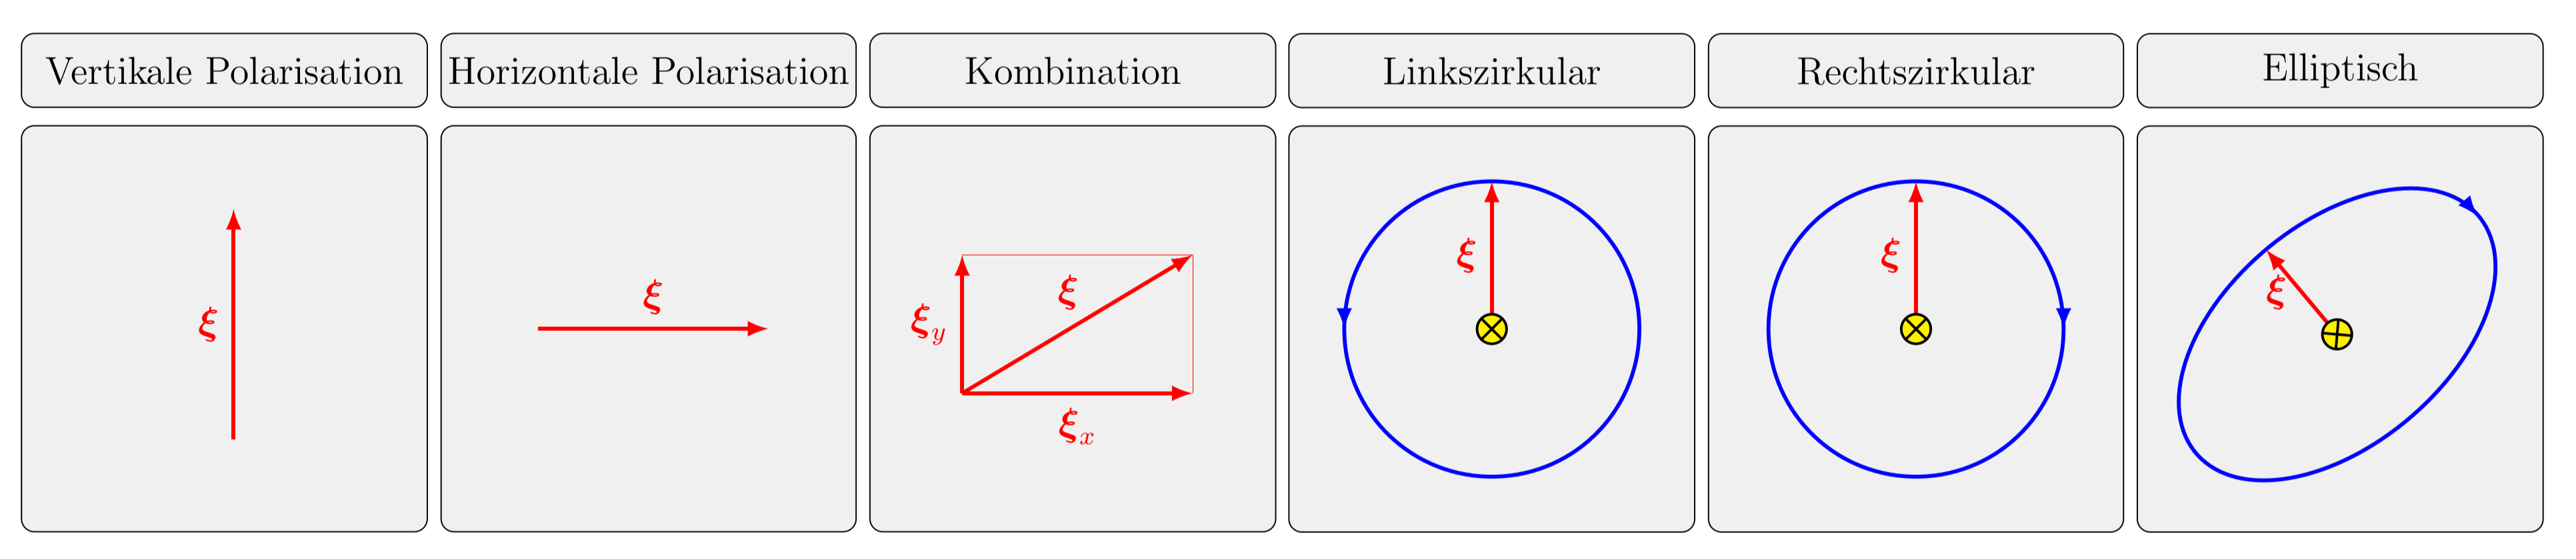
\includegraphics[width=17.8cm]{polarisation.png}}\\
				
				\rowcolor[rgb]{1,1,1}
				\textbf{Gesetzt von Malus} Polarisationsfilter & $\displaystyle I=I_{0} \cdot \cos ^{2}(\alpha)$ & $\alpha$ Polarisationswinkel \qquad\qquad\qquad $I_0$ Intensität \\[5pt]
				
				
				\rowcolor[rgb]{0.91,0.91,0.91}
				\textbf{Mittlere harmonische Energiedichte}  über Periode T  & $\displaystyle\left\langle\frac{\mathrm{d} W}{\mathrm{~d} V}\right\rangle=\frac{1}{T} \int_{0}^{T} \frac{\mathrm{d} W}{\mathrm{~d} V}(x, t) \mathrm{d} t=\frac{1}{2} \rho \omega^{2} A^{2}$&
				Energie pro Zeiteinheit und pro Flächeneinheit \\[10pt]
				
				\rowcolor[rgb]{1,1,1}
				\textbf{Mittlere Intensität} harmonische Welle  & $\displaystyle \langle I\rangle=\frac{1}{2} \rho \omega^{2} A^{2} v=\frac{1}{2} \rho \frac{\omega^{3}}{k} A^{2}= \frac{1}{2} \rho \sqrt{\frac{F}{\rho \pi R^{2}}} \omega^{2} A^{2} \propto \sqrt{\rho} A^{2}$&
				Energie pro Zeiteinheit und pro Flächeneinheit \\[20pt]
				
				\rowcolor[rgb]{0.91,0.91,0.91}
				\textbf{Poynting-Theorem}  Poynting-Vektor:   & $\displaystyle \mathbf{S}=\frac{\mathrm{d}^{2} W}{\mathrm{~d} a \mathrm{~d} t} \frac{\mathrm{d} \vec{a}}{|\mathrm{~d} \vec{a}|}$\qquad , \qquad
				$\displaystyle \mathbf{S}=\mathbf{E} \times \mathbf{H}$&$\displaystyle[S]=\frac{\mathrm{W}}{\mathrm{m}^{2}}$
				\\
				
				
M				&$\displaystyle -\frac{d}{d t} \int_{V}\left(w_{e}+w_{m}\right) d v=\int_{V} p d v+\int_{A=\partial V} \mathbf{S} \cdot d \mathbf{s}$&  $I:=|\vec{S}|$ (Intsensität) \\[10pt]
				
				\rowcolor[rgb]{1,1,1}
				\textbf{Beispiel}  Poyting Vector Ohmischer-Widerstand   &$\displaystyle|\mathbf{S}|=|\mathbf{E} \times \mathbf{H}|=\frac{U \cdot I}{2 \pi R l}$ Integral Mantelfläche
				$\displaystyle P=\oint_{M} \vec{S} \cdot \mathrm{d} \vec{A}=-\frac{U \cdot I}{2 \pi R l} \cdot 2 \pi R l=-U \cdot I$  & elt. Feldstärke $\displaystyle |\vec{E}|=\frac{U}{l}$ ,\qquad mag. Feldstärke$|\displaystyle\vec{H}|=\frac{I}{2 \pi R}$ \\[20pt]

			
			\rowcolor[rgb]{0.91,0.91,0.91}
			\textbf{Energietransport} \qquad kinetische Energiedichte   & $\displaystyle \frac{\mathrm{d} T}{\mathrm{~d} V}=\frac{1}{2} \rho\left(\frac{\partial \xi}{\partial t}\right)^{2}=\frac{1}{2} \rho v^{2}\left(\frac{\mathrm{d} \xi}{\mathrm{d}(x-v t)}\right)^{2}$& Energie $\mathrm{d} T$ \qquad gilt nur für mechanische Wellen
			\\
			elastische Energiedichte & $\displaystyle \frac{\mathrm{d} E_{e l}}{\mathrm{~d} V}=\frac{1}{2} E\left(\frac{\partial \xi}{\partial x}\right)^{2}=\frac{1}{2} S\left(\frac{\partial \xi}{\partial x}\right)^{2}=\frac{\mathrm{d} T}{\mathrm{~d} V}$& Bei Superposition Energien nicht addieren!\\[5pt]
				
			Gesamtenergiedichte &$\displaystyle \frac{\mathrm{d} W}{\mathrm{~d} V}=\frac{\mathrm{d} T}{\mathrm{~d} V}+\frac{\mathrm{d} E_{e l}}{\mathrm{~d} V}=\rho v^{2}\left(\frac{\mathrm{d} \xi}{\mathrm{d}(x-v t)}\right)^{2}=\rho v^{2} f^{\prime 2}$& $\xi(x, t)=f(u)$ mit  $u=x-v t$\qquad $\displaystyle f^{\prime 2}=\frac{\partial f}{\partial u}$ \\	[20pt]
				
			\end{tabular}\\[5pt]
			\hline
		\end{tabular}
	
	
	\begin{tabular}{ | c   p{18cm} |}
	\hline
	\cellcolor{black}\rotcell{\large\textbf{\textcolor{white}{Wellen}}}  &
	\setlength{\extrarowheight}{10pt}			
	\begin{tabular}{L{5cm} L{7cm} L{5cm}}
		
		\rowcolor[rgb]{1,1,1}
		&&\\[-15pt]
		\textbf{Superposition} \qquad \qquad Harmonische Wellen &
		\multicolumn{2}{l}{\parbox{8cm}{$\displaystyle \xi=\underbrace{A \sin (k x-\omega t)}_{\xi_{1}(x, t)}+\underbrace{A \sin (k(x+\Delta x)-\omega t+\delta)}_{\xi_{2}(x, t)}= \underbrace{2 A \cos \left(\frac{1}{2}(\delta+k \Delta x)\right)}_{\text {Amplitude }} \underbrace{\sin \left(k x-\omega t+\frac{1}{2}(\delta+k \Delta x)\right)}_{\text {harmonische Welle }}$ }  } \\[10pt]
		
		Kontruktive/Destruktive Interferenz&$\frac{1}{2}(\delta+k \Delta x)=n \pi$ \quad $\frac{1}{2}(\delta+k \Delta x)=\left(n+\frac{1}{2}\right) \pi$& \\
	
		\rowcolor[rgb]{0.91,0.91,0.91}
		\textbf{Reflexion/Transmission} Auftreffend Welle& $\displaystyle\xi_{A}=A e^{i\left(k_{1} x-\omega t\right)}$ \qquad\qquad \qquad Transversal&  $\displaystyle k_{2}=\omega \sqrt{\frac{\rho_{2}}{S_{2}}}$, $ \displaystyle \alpha=\sqrt{\frac{S_{2} \rho_{2}}{S_{1} \rho_{1}}}$\\
		Reflektierte Welle&	$\displaystyle\xi_{R}=R e^{i\left(-k_{1} x-\omega t+\delta_{R}\right)}$ \qquad\qquad Longitudinal& $\displaystyle k_{2}=\omega \sqrt{\frac{\rho_{2}}{E_{2}}}$,$\displaystyle \alpha=\sqrt{\frac{E_{2} \rho_{2}}{E_{1} \rho_{1}}}$ \\
		Transmitierte Welle&$\displaystyle \xi_{T}=T e^{i\left(k_{2} x-\omega t+\delta_{T}\right)}$&  gesucht: $\displaystyle R,T,\delta_{R}, \delta_{T}, k_{2} $ \\
		Phase &$\delta_{R}=0 \qquad \delta_{R}=\pi \qquad \delta_{T}=0$&\\
		Amplitude &$R=\frac{1-\alpha}{1+\alpha} A \quad R=-\frac{1-\alpha}{1+\alpha} A$\qquad $T=\frac{2 A}{1+\alpha}$&$(R \geq 0)$ \\
		\textbf{Spezialfall} \qquad festes (Seil-)Ende $(\alpha \rightarrow \infty)$& $\displaystyle\underbrace{\delta R=\pi}_{\pi \text { Phasensprung }}$\quad$\displaystyle\lim _{\alpha \rightarrow \infty} R=A$\quad $\displaystyle \lim _{\alpha \rightarrow \infty} T=0$ &($\alpha = 0$ nur bei übergang zu Vakuum. mech. Welle
		kann nicht ins Vakuum, d.h $T = 0$ statt $T = 2A$)\\
		loses (Seil-) Ende $(\alpha \rightarrow 0)$&$\displaystyle\underbrace{\delta R=0}_{\text {kein Phasensprung }}$ , $\displaystyle \lim _{\alpha \rightarrow \infty} R=A$, $\displaystyle\lim _{\alpha \rightarrow \infty} T=0$&\\[10pt]
	
		\rowcolor[rgb]{1,1,1}
		&&\\[-15pt]	
		\textbf{Stehende Wellen} \qquad \qquad gegeenlaufende Harmonische Wellen &
		\multicolumn{2}{l}{\parbox{8cm}{$\displaystyle \xi(x,t)=\underbrace{A \sin (k x-\omega t)}_{\xi_{1}(x, t)}+\underbrace{A \sin (kx+\omega t+\delta)}_{\xi_{2}(x, t)}= \underbrace{2 A \sin \left(kx+\frac{\delta}{2}\right)}_{\text {Amplitude }} \underbrace{\cos \left(\omega t+\frac{\delta}{2}\right)}_{\text {harmonische Welle }}$ }  } \\[10pt]
		
		Saite fest-fest ($n$-te Normalschwingung) &$\xi_{n}(x, t)=A_{n} \sin \left(\frac{n \pi}{l} x\right) \cos \left(\frac{n \pi}{l} v t+\varphi_{n}\right)$&\\
		Saite fest-offen&$\displaystyle\xi_{n}(x, t)=A_{n} \sin \left(\frac{2 n+1}{2} \frac{\pi}{l} x\right) \cos \left(\frac{2 n+1}{2} \frac{\pi}{l} v t+\varphi_{n}\right)$&\\
		
		
		
		\rowcolor[rgb]{0.91,0.91,0.91}
		&&\\[-15pt]
		\textbf{Prinzip von Huygens}&\multicolumn{2}{l}{\parbox{12cm}{Jeder Punkt einer bestehenden Wellenfläche (bzw. Wellenfront) wird als Zentrum einer neuen kugelförmigen Elementarwelle aufgefasst. Die Umhüllende dieser Elementarwellen ergibt dann die Wellenfront zu einem späteren Zeitpunkt.}}
		\\[20pt]
		
		\rowcolor[rgb]{1,1,1}
		\textbf{Einzelspalt} &
		$\displaystyle\langle I\rangle \propto A^{2} \frac{\sin ^{2}\left(\frac{\Delta \varphi}{2}\right)}{\left(\frac{\Delta \varphi}{2}\right)^{2}}$
		mit $\quad \Delta \varphi=k d \sin (\alpha)$ &$\Delta \varphi$ Phasendifferenz	 \\[10pt]
		
		
		\textbf{Beispiel}&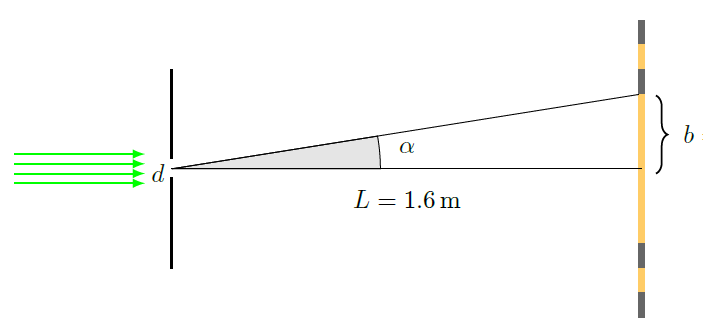
\includegraphics[width=7cm]{spalt.png}& $\langle I\rangle \sim A^{2} \frac{\sin ^{2}\left(\frac{1}{2} \Delta \varphi\right)}{\left(\frac{1}{2} \Delta \varphi\right)^{2}}, \quad$ mit $\quad \Delta \varphi=2 \pi \frac{d}{\lambda} \sin \alpha$ $I$ verschwindet bei $\frac{1}{2} \Delta \varphi=n \pi, n \in \mathbb{N}$ \qquad $\Rightarrow d=n \frac{\lambda}{\sin \alpha}=n \frac{\lambda}{b/L}$\\
		
		
	
		
	\end{tabular}\\[5pt]
	\hline
\end{tabular}	
	
	
	\begin{tabular}{ | c   p{18cm} |}
		\hline
		\cellcolor{black}\rotcell{\large\textbf{\textcolor{white}{Wellen}}}  &
		\setlength{\extrarowheight}{10pt}			
		\begin{tabular}{L{5cm} L{7cm} L{5cm}}
			
			&&\\[-15pt]
			\textbf{Snellius’sche Brechungsgesetz} &
			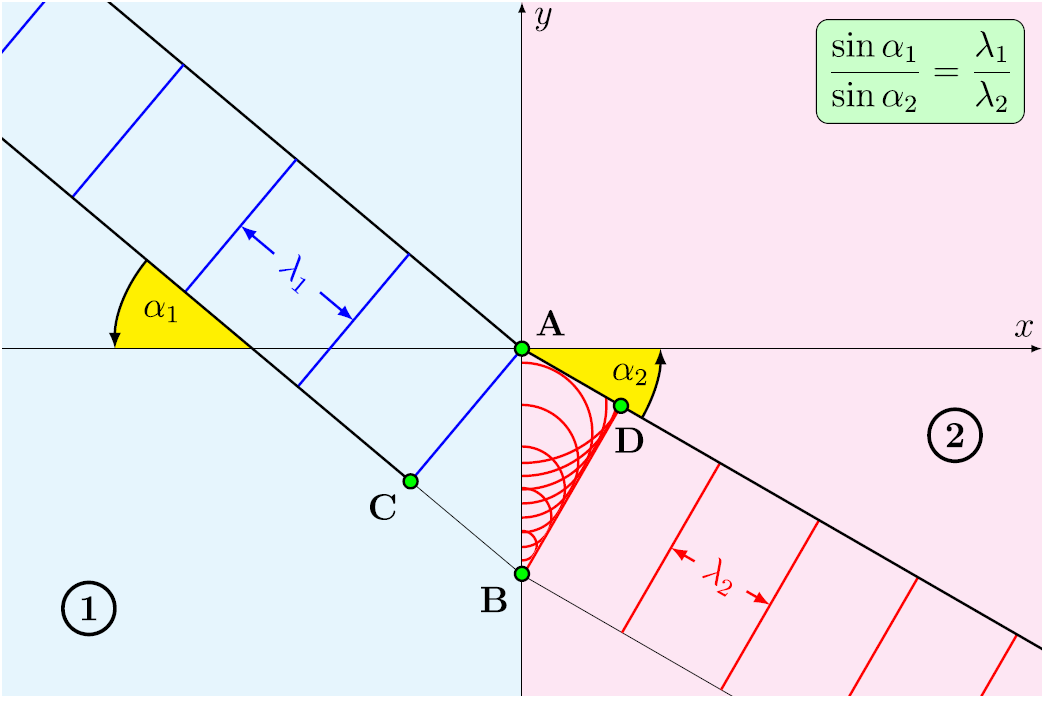
\includegraphics[width=7cm]{huygens2.png}&$\displaystyle\frac{\sin \left(\alpha_{1}\right)}{\sin \left(\alpha_{2}\right)}=\frac{v_{1}}{v_{2}}=\frac{\lambda_{1}}{\lambda_{2}}$ \\[10pt]
			
						
			\rowcolor[rgb]{0.91,0.91,0.91}
			&&\\[-15pt]
			\textbf{Fermat’sches Prinzip}&\multicolumn{2}{l}{\parbox{12cm}{Nach dem Fermat’schen Prinzip läuft eine Welle bei Reflexion und Brechung, stets jenen Weg, für den die Laufzeit einer Phasenfläche $\Phi$ zwischen zwei Punkten minimal wird.}}
			\\[20pt]
			
			
			
			\rowcolor[rgb]{1,1,1}
			&&\\[-15pt]
			\textbf{Dopplereffekt} &
			$\displaystyle f_{B}=\frac{c+v_{b}}{c-v_{q}} f_{q}$  \qquad $c_{\text{Luft}}= 340m/s$ &
		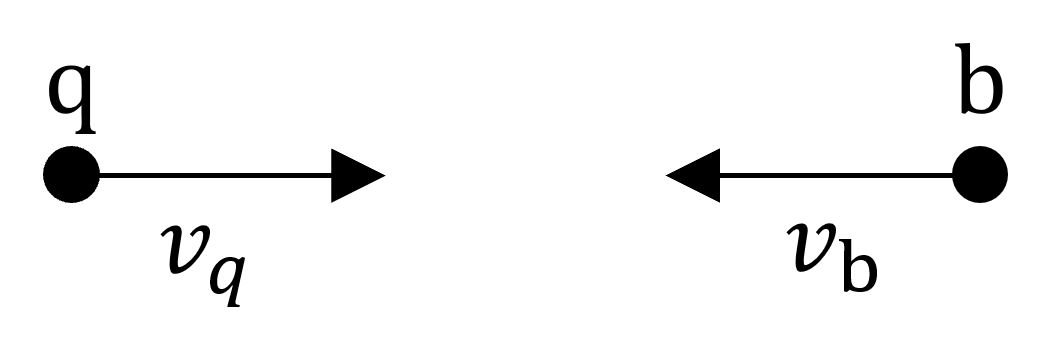
\includegraphics[width=3cm]{doppler.jpg} \\[10pt]
			
			\rowcolor[rgb]{0.91,0.91,0.91}
			\textbf{Schockwelle} & 
			$\displaystyle \vartheta=\arcsin \left(\frac{u}{v_{Q}}\right)$ & 
			$\displaystyle \vartheta$ Halber Öffnungswinkel Machscher Kegel \\[10pt]
			
			
			
			
		\end{tabular}\\[5pt]
		\hline
	\end{tabular}	
	

				
			
\begin{tabular}{ | c   p{18cm} |}
				\hline
				%\rowcolor{blue!30}
				\cellcolor{black}\rotcell{\large\textbf{\textcolor{white}{Maxwell-Gleichungen}}}  &
				\setlength{\extrarowheight}{5pt}	
				
				\begin{tabular}{L{4cm} R{4.2cm} C{0.5cm} L{6.3cm} L{0.9cm}}
					&&&&\\[-10pt]
					
					\textbf{Physikalisches gaußsches Gesetz}&
					$\displaystyle \operatorname{div} \vec{D}=\vec{\nabla} \cdot \vec{D}=\rho$&$\displaystyle \Longleftrightarrow$& $\displaystyle \oint_{\partial V} \vec{D} \cdot \mathrm{d} \vec{A}=\iiint_{V} \rho \mathrm{d} V=Q(V)$ & Gauss\\[10pt]
					
				\multicolumn{2}{l}{\parbox{8.2cm}{Das $\displaystyle \vec {D}$-Feld ist ein Quellenfeld. Die Ladung (Ladungsdichte ${\displaystyle \rho }$) ist Quelle des elektrischen Feldes.}}&&\multicolumn{2}{l}{\parbox{6.5cm}{Der (elektrische) Fluss durch die geschlossene Oberfläche $\displaystyle \partial V$ eines Volumens $V$ ist direkt proportional zu der elektrischen Ladung in seinem Inneren.}}\\	[10pt]
					
					
				\rowcolor[rgb]{0.91,0.91,0.91}
				\textbf{Quellenfreiheit des B-Feldes}&
				$\displaystyle\operatorname{div} \vec{B}=\vec{\nabla} \cdot \vec{B}=0 $&$\Longleftrightarrow$&$\displaystyle \oint_{\partial V} \vec{B} \cdot \mathrm{d} \vec{A}=0$ & Gauss\\[10pt]
				
				\multicolumn{2}{l}{\parbox{8.2cm}{Das $\vec {B}$-Feld ist quellenfrei. Es gibt keine magnetischen Monopole.}}&&
				\multicolumn{2}{l}{\parbox{6.5cm}{Der magnetische Fluss durch die geschlossene Oberfläche eines Volumens ist gleich der magnetischen Ladung in seinem Inneren, nämlich Null, da es keine magnetischen Monopole gibt.}}\\	[10pt]
				
				
					
					
					
				\rowcolor[rgb]{1,1,1}	
				\textbf{Induktionsgesetz}&
				$\displaystyle\operatorname{rot} \vec{E}=\vec{\nabla} \times \vec{E}=-\frac{\partial \vec{B}}{\partial t} $&$\Longleftrightarrow$&$\displaystyle \oint_{\partial A} \vec{E} \cdot \mathrm{d} \vec{s}=-\iint_{A} \frac{\partial \vec{B}}{\partial t} \cdot \mathrm{d} \vec{A}$ & Stokes\\[10pt]
				
				
				\multicolumn{2}{l}{\parbox{8.2cm}{Jede Änderung des $\vec {B}$-Feldes führt zu einem elektrischen Gegenfeld. Die Wirbel des elektrischen Feldes sind von der zeitlichen Änderung der magnetischen Flussdichte abhängig.}}&&
				\multicolumn{2}{l}{\parbox{6.5cm}{Die (elektrische) Zirkulation über der Randkurve $\partial A$ einer Fläche $A$ ist gleich der negativen zeitlichen Änderung des magnetischen Flusses durch die Fläche.}}\\[10pt]	
				
					
				\rowcolor[rgb]{0.91,0.91,0.91}
				\textbf{Durchflutungsgesetz}&
				$\displaystyle \operatorname{rot} \vec{H}=\vec{\nabla} \times \vec{H}=\vec{j}_{1}+\frac{\partial \vec{D}}{\partial t}$&$ \Longleftrightarrow$&$\displaystyle \oint_{\partial A} \vec{H} \cdot \mathrm{d} \vec{s}=\iint_{A} \vec{j}_{1} \cdot \mathrm{d} \vec{A}+\iint_{A} \frac{\partial \vec{D}}{\partial t} \cdot \mathrm{d} \vec{A}$ & Stokes\\[10pt]
				
				\multicolumn{2}{l}{\parbox{8.2cm}{Die Wirbel des Magnetfeldes hängen von der Leitungsstromdichte $\vec {j}_{\mathrm {l}}$ und von der elektrischen Flussdichte $\vec {D}$ ab. Die zeitliche Änderung von $\vec {D}$ wird auch als Verschiebungsstromdichte $\vec {j}_{\mathrm {v}}$ bezeichnet und ergibt als Summe mit der Leitungsstromdichte die totale Stromdichte $\vec {j}_{\text{total}}=\vec {j}_{\mathrm {l} }+\vec {j}_{\mathrm {v}}$}}&&
				\multicolumn{2}{l}{\parbox{6.5cm}{Die magnetische Zirkulation über der Randkurve $\partial A$ einer Fläche $A$ ist gleich der Summe aus dem Leitungsstrom und der zeitlichen Änderung des elektrischen Flusses durch die Fläche.}}\\[10pt]	
				
					
				\end{tabular}\\
				\hline
			
		\end{tabular}

	%Elektro / Magnetismus
	
		\begin{tabular}{ | c   p{18cm} |}
			\hline
			%\rowcolor{blue!30}
			\cellcolor{black}\rotcell{\large\textbf{\textcolor{white}{Elektrostatik}}}  &
			\setlength{\extrarowheight}{10pt}	
					
			\begin{tabular}{L{5cm} L{6.5cm} L{5.3cm}}
				
			\textbf{Elektrische Feldstärke}&
			$\displaystyle \vec{E}=\lim _{q \rightarrow 0} \frac{\vec{F}}{q} \qquad\qquad \vec{F}=q \vec{E}$
			&
			$\displaystyle[E]=\frac{\mathrm{V}}{\mathrm{m}}$ \\[5pt]
			für $n$ Ladungen&$\displaystyle \vec{E}(\vec{r}) = \frac{1}{4\pi\varepsilon_0} \sum_{i=1}^{n} \frac{q_i}{|\vec{r}-\vec{r}_i|^3}(\vec{r}-\vec{r}_i)$ &\\
			Ladungsverteilung&$\displaystyle	\vec{E}(\vec{r}) = \frac{1}{4\pi\varepsilon_0} \iiint_{\mathbb{R}^3} \frac{\rho(r')}{|\vec{r}-\vec{r}'|^3}(\vec{r}-\vec{r}') \diff x' \diff y' \diff z' $&(Ladungsdichte $\rho$)\\
			

			\textbf{Punktladung}&
			$\displaystyle \vec{E}(\vec{r}) = \frac{1}{4\pi\varepsilon_0} \frac{q\hat{r}}{r^2}$ & \\
			
			\textbf{Kugeloberfläche}&
			$\displaystyle \vec{E}(\vec{r})= \begin{cases}0 \qquad\qquad r<R \\ \displaystyle\frac{1}{4 \pi \varepsilon_{0}} \frac{q \hat{r}}{r^{2}} \qquad r>R\end{cases}$&
			
			\textbf{$\infty$-Draht}\qquad $\displaystyle \vec{E}(\vec{r})= \frac{\lambda}{2\pi\varepsilon_0r}$\\
		
			\textbf{$\infty$-Zylinder}&
			$\displaystyle \vec{E}(\vec{r})= \begin{cases}0 \qquad\qquad r<R \\ \displaystyle \frac{\lambda \hat{r}}{2 \pi \varepsilon_{0} r} \qquad r>R\end{cases}$&
			
	
			\textbf{$\infty$-Ebene}\qquad
			$\displaystyle \vec{E}(\vec{r})=\frac{\sigma}{2\varepsilon_0}$\\
			
			
			
							
			\rowcolor[rgb]{0.91,0.91,0.91}
			\textbf{Coulombsches Gesetz} &
			$\displaystyle \vec{F}_{21}=k \frac{q_{1} q_{2}}{r_{21}^{2}} \hat{r}_{21}$&
			 $\displaystyle k=\frac{1}{4 \pi \varepsilon_{0}}$\\[10pt]
				
				
			\rowcolor[rgb]{1,1,1}
			\textbf{Earnshaw-Theorem}&\multicolumn{2}{l}{\parbox{10cm}{Kein System stationärer Ladung ist in einem stabilen Gleichgewicht unter der alleinigen Wirkung elektrischer Kräfte}}
					\\[10pt]
				
			\rowcolor[rgb]{0.91,0.91,0.91}
			\textbf{Elektrische Flussdichte} 	& $D=\epsilon E = \epsilon_0 \epsilon_r E$\qquad$ (\epsilon_r = 1 + \chi_e)$   & $\displaystyle[D]= \frac{C}{m^2}$  \\[5pt]
			
			\rowcolor[rgb]{1,1,1}
			\textbf{Elektrischer Fluss}\qquad\qquad &
			$\displaystyle   \Psi_D = \int_{A}{ \vec{D}\cdot \diff\vec{s}}$\qquad $\displaystyle\Psi_E = \int_{A}{ \epsilon_0\vec{E}\cdot \diff\vec{s}}$&$[\Psi]= C (Coulomb) = As$ \\
			
			bei geschlossener Oberfläche& $\displaystyle \Psi_D=\oint_{\text{Hülle}} \vec{D} \cdot \mathrm{d} \vec{s}=Q_{umschlossen}$&
			$\Psi=CU=Q$\\[10pt]
			
			\rowcolor[rgb]{0.91,0.91,0.91}
			\textbf{Elektrischer Fluss} \qquad\qquad im Vakuum	&\multicolumn{2}{l}{
			$\displaystyle \diff \Phi = \vec{E}\cdot \diff\vec{a} \qquad \Rightarrow \qquad \Phi =\frac{\Psi}{\epsilon_0}= \int_{\del V} \vec{E}\cdot \diff\vec{a}$} \\[5pt]
			
			\rowcolor[rgb]{1,1,1}
			\textbf{Gaussches Gesetz}&
			$\displaystyle \Phi = \int_{\del V}\epsilon_0 \vec{E}\cdot \diff\vec{a} = \int_V \rho \diff V = \sum_V q=Q$&$\displaystyle \Psi_D=\oint_{\text{Hülle}} \vec{D} \cdot \mathrm{d} \vec{s}=Q_{frei}$ \\[5pt]
					
			\rowcolor[rgb]{0.91,0.91,0.91}
			\textbf{Energiedichte}	&
			$\displaystyle w = \frac{\diff W}{\diff V} = \frac{\varepsilon_0}{2}E^2$&\\[5pt]
			
			\rowcolor[rgb]{1,1,1}
			\textbf{Potentielle Energie}&
			$\displaystyle W =\int_V w \diff V = \int_V \frac{\varepsilon_0}{2}E^2 \diff V$&\\[5pt]
			
			\rowcolor[rgb]{0.91,0.91,0.91}
			\textbf{E-Feld konservativ}&
			$\displaystyle \oint \vec{E} \cdot \diff\vec{s} =0 \qquad \Leftrightarrow \qquad \vec{E} = -\nabla \phi$&\\[5pt]
			
			\rowcolor[rgb]{1,1,1}
			\textbf{Potentialdifferenz}&
			$\displaystyle U_{AB} =\phi(A) - \phi(B) = \int_{A}^{B} \vec{E}\cdot\diff\vec{s}$& $[U]=V$ \\[5pt]
			
			\rowcolor[rgb]{0.91,0.91,0.91}
			\textbf{Potential mehrere Ladungen}&
			$\displaystyle \phi(\vec{r}) = \frac{1}{4\pi\varepsilon_0} \iiint_{\mathbb{R}^3} \frac{\rho(\vec{r'})}{|\vec{r}-\vec{r'}|}\diff x' \diff y' \diff z'$&\\[5pt]
			
			
			
			\rowcolor[rgb]{1,1,1}
			\textbf{Potentielle Energie }\qquad \qquad einer Ladungsverteilung ($\rho$)&
			$\displaystyle	W = \frac{1}{2}\iiint_{\mathbb{R}^3} \phi(\vec{r})\rho(\vec{r})\diff x \diff y \diff z
			$&\\[5pt]
			
			
			\rowcolor[rgb]{0.91,0.91,0.91}
			& $\displaystyle U_{BA} = E\Delta z \quad$ & Plattenkondensator\\[-2pt]
			\textbf{Potentiale einfacher Ladungsverteilung}& $\displaystyle U_{BA} = \frac{1}{4\pi\varepsilon_0}\frac{q}{r}$ & Punktladung\\[-1pt]
			& $\displaystyle U_{BA} = \frac{1}{4\pi\varepsilon_0}\frac{q}{\sqrt{x^2 + R^2}}$ & Ringladung\\[-1pt]
			& $\displaystyle U_{BA} = \frac{\sigma}{2\varepsilon_0}\left( \sqrt{x^2+R^2}-x\right)$  & Scheibe\\[5pt]
			

	
			\end{tabular}\\
			\hline
		\end{tabular}
	
	
	
	\begin{tabular}{ | c   p{18cm} |}
		\hline
		\cellcolor{black}\rotcell{\large\textbf{\textcolor{white}{Elektrische Leiter}}}  &
		\setlength{\extrarowheight}{10pt}	
		
		\begin{tabular}{L{5cm} L{6.5cm} L{5.3cm}}
			&&\\
			
			\rowcolor[rgb]{1,1,1}
			\multicolumn{3}{l}{\parbox{17cm}{\begin{itemize}
						\item[(1)] Das elektrische Potential $\phi$ besitzt im Innern und auf der Oberfläche denselben Wert (Oberflächen sind Äquipotentialflächen).
						\item[(2)] Das E-Feld verschwindet im Innern und ist ausserhalb orthogonal auf die Oberfläche
						\[
						\vec{E} = \frac{\sigma}{\varepsilon_0}\hat{n}
						\]
						\begin{flushright}
							($\sigma$ lokale Flächenladungsdichte,\\
							$\vec{n}$ Normalenvektor)
						\end{flushright}
						\item[(3)] Je kleiner Krümmung der Oberfläche, umso grösser die Oberflächeladungsdichte $\sigma$.
						\item[(4)] Die Gesamtladung ist durch Integration über die Oberfläche gegeben
						\[
						q = \int_A \sigma \diff a = \varepsilon_0\int_A E\diff a
						\]
			\end{itemize}}}
			\\[70pt]

			
		
		\end{tabular}\\[10pt]
		\hline
	\end{tabular}\\

	
	
	
	
	

		\begin{tabular}{ | c   p{18cm} |}
		\hline
		\cellcolor{black}\rotcell{\large\textbf{\textcolor{white}{Magnetostatik}}}  &
		\setlength{\extrarowheight}{10pt}	
		
		\begin{tabular}{L{5cm} L{6.5cm} L{5.3cm}}
			&&\\[-20pt]
			\rowcolor[rgb]{1,1,1}
			
			
			\textbf{Magnetische Flussdichte} \qquad\qquad\qquad Gesetzt von Biot-Savart Ladungsdichte&$\displaystyle \mathbf{B}=\frac{\mu_{0}}{4 \pi} \int_{V} \frac{(\mathbf{J} d v) \times \hat{\mathbf{R}}}{R^{2}}=\frac{\mu_{0}}{4 \pi} \int_{L} \frac{(I d \mathbf{l}) \times \hat{\mathbf{R}}}{R^{2}} $&$\displaystyle [B]=\mathrm{T}=\frac{\mathbf{W b}}{\mathrm{m}^{2}}$\\[5pt]
			
			
			\rowcolor[rgb]{0.91,0.91,0.91}
			\textbf{Magnetische Feldstärke} \qquad\qquad Magnetische Hilfsgrösse&$\displaystyle \mathbf{H}=\frac{\mathbf{B}}{\mu_{0}}-\mathbf{M} $&$\displaystyle \left[H\right]=\frac{\mathrm{A}}{\mathrm{m}}$\\[5pt]
	
			\rowcolor[rgb]{1,1,1}
			\textbf{Magn. Materialgleichung} \qquad\qquad\qquad magn. Permeabilität$\mu$&
			$\displaystyle \mathbf{B}=\mu \mathbf{H}=\mu_{0} \mu_{r} \mathbf{H}=\mu_{0}(\mathbf{H}+\mathbf{M}) $&$\displaystyle \left(\mu_{r}=1+\chi_{m}\right)$\\[5pt]
			
				\rowcolor[rgb]{0.91,0.91,0.91}
			\textbf{ Magnet. Vektorpotential} &$\displaystyle \mathbf{A}=\frac{\mu_{0}}{4 \pi} \int_{V} \frac{\mathbf{J} d v}{R}=\frac{\mu_{0}}{4 \pi} \int_{L} \frac{I d \mathbf{l}}{R}$&$\left[ A\right ]= Wb/m$ (nicht Fläche A)\\[5pt]
			
			\rowcolor[rgb]{1,1,1}
			\textbf{Magnetische Spannung} \qquad\qquad\qquad und Umlaufsspannung$\mu$&
			$\displaystyle V_{m}=\int_{L} \mathbf{H} \cdot d \mathbf{l}, \quad \stackrel{\circ}{V}_{m}=\oint_{C} \mathbf{H} \cdot d \mathbf{l}$
			& $\displaystyle \left[V_m\right]=A$\\[5pt]
			
			
			\rowcolor[rgb]{0.91,0.91,0.91}
			\textbf{Magnet. Dipolmoment}\qquad\qquad (einer Stromschleife) &$\displaystyle \mathbf{m}=\hat{\mathbf{n}} I A \quad(\hat{\mathbf{n}} \perp A)  \Rightarrow \quad \mathbf{T}=\mathbf{m} \times \mathbf{B} $&$[m]=\mathrm{A} \mathrm{m}^{2}$\\[5pt]
			
			
			\rowcolor[rgb]{1,1,1}
			\textbf{Magnetisierung } \qquad\qquad\qquad (im linearen Bereich)&
			$\displaystyle \mathbf{M}=\chi_{m} \mathbf{H}=\frac{d}{d v}\left[\sum_{n} \mathbf{m}_{n}\right]_{\text {in } d v}=N_{m} \mathbf{m}$
			& $\displaystyle [m]=\frac{\mathrm{A}}{\mathrm{m}} $\\[5pt]
			
			
			
			\rowcolor[rgb]{0.91,0.91,0.91}
			\textbf{Magnetischer Fluss}\qquad\qquad und magn. Widerstand $R_m$ &$\displaystyle \Phi=\int_{A} \mathbf{B} \cdot d \mathbf{s}=\oint_{C=\partial A} \mathbf{A} \cdot d \mathbf{l}=\frac{V_{m}}{R_{m \mid}}=V_{m} \Lambda$&$[\Phi]=Wb=Tm^2$\\[5pt]
					
					
			\rowcolor[rgb]{1,1,1}
			\textbf{Induktivität } \qquad\qquad\qquad Selbst- \& Gegeninduktivität&
			$\displaystyle L=\frac{\Phi_{1}}{I_{1}}=L_{a}+L_{i}, \quad M=\frac{\Phi_{2}}{I_{1}}=k \sqrt{L_{1} L_{2}}$& $\displaystyle [L]=[M]=H$ \qquad (nicht Magnet.M!) \\[5pt]		
				
			\rowcolor[rgb]{0.91,0.91,0.91}
			\textbf{Gespeicherte Energie}\qquad\qquad einer Induktivität &$\displaystyle W_{m}=\frac{1}{2} L I^{2}=\frac{1}{2} \frac{\Phi^{2}}{L}$&$\displaystyle [W_m]=J=Ws$\\[5pt]	
			
			
			
			\rowcolor[rgb]{1,1,1}
			\textbf{Energiedichte } \qquad\qquad\qquad des magnetischen Felds&
			$\displaystyle w_{m}=\frac{d W_{m}}{d v}=\frac{1}{2} \mathbf{B} \cdot \mathbf{H}=\frac{1}{2} \mu H^{2}=\frac{B^{2}}{2 \mu}$& $\displaystyle [w_m]=\frac{J}{m^3}$ \\[5pt]	
					
					
				
			\rowcolor[rgb]{0.91,0.91,0.91}
			\textbf{Magnetkraft}\qquad\qquad Maxwellsche Zugkraftformel &$\displaystyle \mathbf{F}=\frac{d W_{m}}{d l} \hat{\mathbf{l}}=\frac{B^{2} A}{2 \mu_{0}} \hat{\mathbf{n}} \quad(\hat{\mathbf{n}} \perp A)$&$\displaystyle [F]=N$\\[5pt]
			
			\rowcolor[rgb]{1,1,1}
			\textbf{Ampèresche Gesetze} \qquad\qquad\qquad Durchflutungssatz $\Theta =\stackrel{\circ}{V}_{m}$&\multicolumn{2}{l}{
			$\displaystyle \oint_{C=\partial A} \mathbf{B} \cdot d \mathbf{l}=\mu_{0} \int_{A} \mathbf{J} \cdot d \mathbf{s}, \quad \oint_{C=\partial A} \mathbf{H} \cdot d \mathbf{l}=\int_{A} \mathbf{J}_{\mathbf{f r e i}} \cdot d \mathbf{s}=\Theta$} \\[5pt]	
		
			\rowcolor[rgb]{0.91,0.91,0.91}
			\textbf{Gausssches Gesetz}\qquad\qquad Flusskontinuität &\multicolumn{2}{l}{
				$\displaystyle \oint_{\text{Hülle}} \mathbf{B} \cdot d \mathbf{s}=0$ \qquad $\Leftrightarrow$\qquad$\displaystyle \sum_{n} \Phi_n =0$ }
			\\[5pt]
					
		\end{tabular}\\
		\hline
	\end{tabular}
		\begin{tabular}{ | c   p{18cm} |}
		\hline
		\cellcolor{black}\rotcell{\large\textbf{\textcolor{white}{Stationäre Strömung}}}  &
		\setlength{\extrarowheight}{10pt}	
		
		\begin{tabular}{L{5cm} L{6.5cm} L{5.3cm}}
			&&\\[-20pt]
			\rowcolor[rgb]{1,1,1}
			\textbf{Stromdichte} \qquad\qquad\qquad Bewegte Ladungsdichte&$\displaystyle \mathbf{J}=\rho \mathbf{v}=\sigma \mathbf{E} $&$ \displaystyle[J]=\frac{\mathrm{A}}{\mathrm{m}^{2}}$\\[5pt]
			
			
			\rowcolor[rgb]{0.91,0.91,0.91}
			\textbf{Elektrische Leitfähigkeit} \qquad\qquad Konduktanz&$\displaystyle\sigma=\underbrace{n_{e} q_{e}}_{\rho} \mu_{e} $&$\displaystyle\left(+n_{p} q_{p} \mu_{p}\right) \quad[\sigma]=\frac{\mathrm{S}}{\mathrm{m}}$\\[5pt]
	
		
		
			\rowcolor[rgb]{1,1,1}
			\textbf{Elektrischer Strom} \qquad\qquad Elektrische Strömung&
			$\displaystyle I=\int_{A} \mathbf{J} \cdot d \mathbf{s}=\left.\frac{d Q}{d t}\right|_{\text {durch } A} \quad(I l=q \mathbf{v}) $&$\displaystyle [I]=\mathbf{A}=\frac{\mathrm{C}}{\mathrm{s}}$ \\[5pt]
			
			
			\rowcolor[rgb]{0.91,0.91,0.91}
			\textbf{Leitwert} \qquad\qquad\qquad (Kehrwert: Widerstand)&$\displaystyle G=\frac{I}{U} \quad \Leftrightarrow \quad R=\frac{1}{G}=\frac{U}{I} $&$\displaystyle [G]=\mathrm{S}=\frac{1}{\Omega}$\\[5pt]
			
			\rowcolor[rgb]{1,1,1}
			\textbf{Leistung} \qquad\qquad\qquad am Widerstand/Leitwert &$\displaystyle P=U I=\frac{U^{2}}{R}=G U^{2}=I^{2} R=\frac{I^{2}}{G} $&$\displaystyle [P]=\mathrm{W}=\frac{\mathrm{J}}{\mathrm{s}}$ \\[5pt]
			
			\rowcolor[rgb]{0.91,0.91,0.91}
			\textbf{Leistungsdichte} \qquad\qquad\qquad des Strömungsfelds&
			$\displaystyle p=\frac{d P}{d v}=\mathbf{J} \cdot \mathbf{E}=\sigma E^{2} $&$\displaystyle [p]=\frac{\mathrm{W}}{\mathrm{m}^{3}}$
			\\[5pt]
			
			
			\rowcolor[rgb]{1,1,1}
			\textbf{Gausssches Gesetz} \qquad\qquad\qquad Kirchhoffscher Knotensatz &\multicolumn{2}{l}{$\oint_{\text {Holle }} \mathbf{J} \cdot d \mathbf{s}=0 \quad \Leftrightarrow \quad \sum_{n} I_{n}=0$ }\\[5pt]
					
		\end{tabular}\\
		\hline
	\end{tabular}
		\begin{tabular}{ | c   p{18cm} |}
		\hline
		\cellcolor{black}\rotcell{\large\textbf{\textcolor{white}{Kondensator}}}  &
		\setlength{\extrarowheight}{10pt}	
		
		\begin{tabular}{L{5cm} L{6.5cm} L{5.3cm}}
			
			\rowcolor[rgb]{1,1,1}
			\textbf{Kapazität}&$\displaystyle C = \frac{Q}{U}$&$\displaystyle[C]= F=\frac{C}{V}$\\[5pt]
			
			
			\rowcolor[rgb]{0.91,0.91,0.91}
			\textbf{Plattenkondensator}& $	{\displaystyle C=\varepsilon _{0}\varepsilon _{\mathrm {r} }\cdot {\frac {A}{d}}}$\qquad$\displaystyle E={\frac {Q}{\varepsilon _{0}\varepsilon _{\mathrm {r} }A}}$   &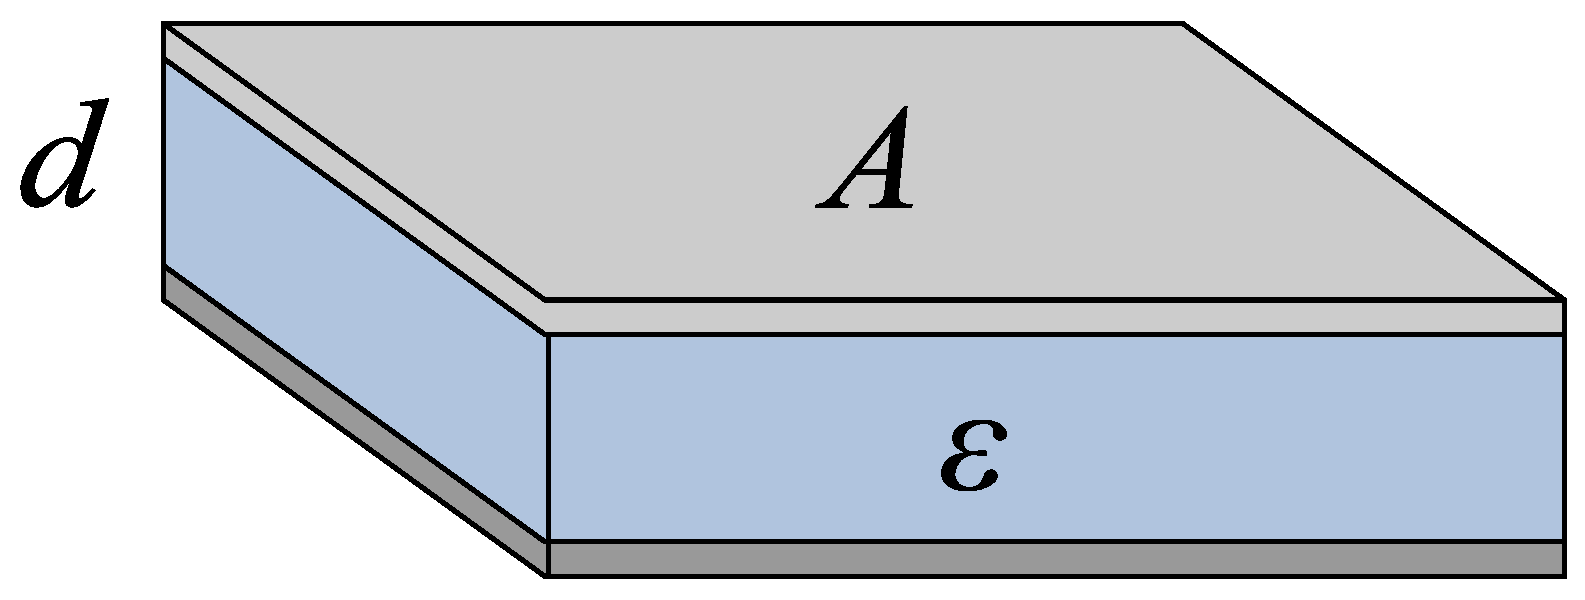
\includegraphics[width=4cm]{platten.pdf}\\
			
			
			
			\rowcolor[rgb]{1,1,1}
			\textbf{Zylinderkondensator}& $	{\displaystyle C=2\pi \varepsilon _{0}\varepsilon _{\mathrm {r} }{\frac {l}{\ln \left({\frac {R_{2}}{R_{1}}}\right)}}}$ \quad $\displaystyle E(r)={\frac {Q}{2\pi rl\varepsilon _{0}\varepsilon _{\mathrm {r} }}}$ &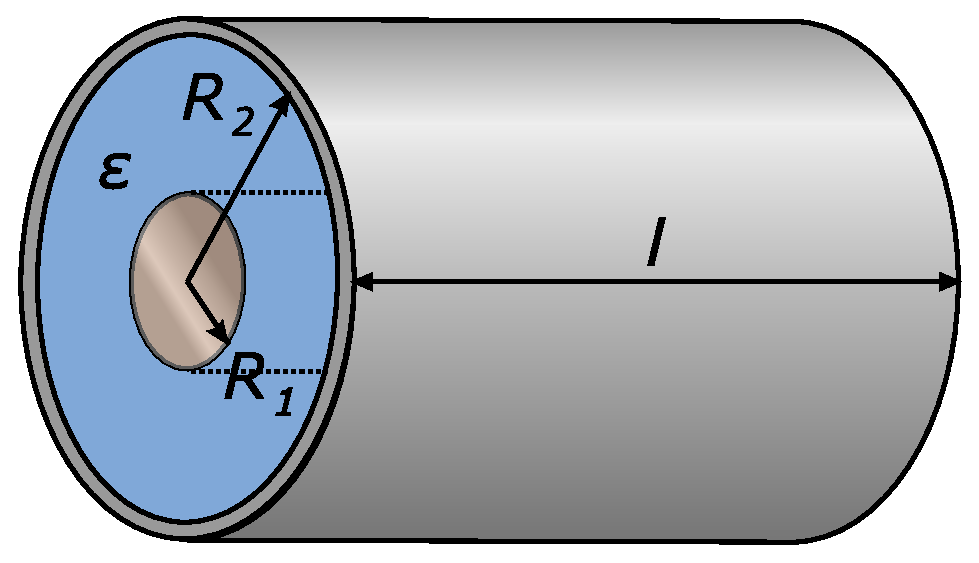
\includegraphics[width=3.5cm]{zylinder.pdf}\\
			
			
			\rowcolor[rgb]{0.91,0.91,0.91}
			\textbf{Plattenkondensator}& $	\displaystyle C=4\pi \varepsilon _{0}\varepsilon _{\mathrm {r} }\left({\frac {1}{R_{1}}}-{\frac {1}{R_{2}}}\right)^{-1}$  \quad
				$\displaystyle E(r)={\frac {Q}{4\pi r^{2}\varepsilon _{0}\varepsilon _{\mathrm {r} }}}$
				 &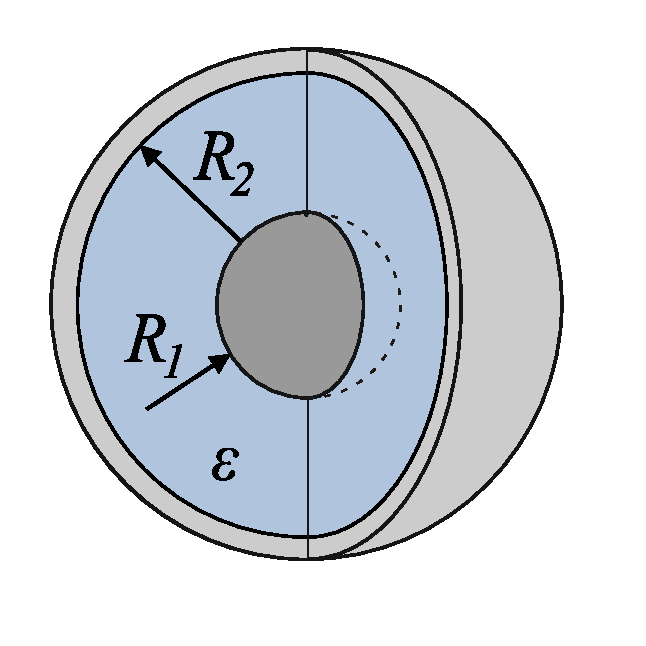
\includegraphics[width=3cm]{kugel.pdf}\\
				 
				 
				 
			\rowcolor[rgb]{1,1,1}
			\textbf{Gespeicherte Energie} \qquad einer Kapazität&	 
			$\displaystyle W_e = \frac{Q^2}{2C} = \frac{CU^2}{2} = \frac{QU}{2}	$ & $\displaystyle [W_e]=J =Ws$
			\\
			
			\rowcolor[rgb]{0.91,0.91,0.91}
			\textbf{Energiedichte} \qquad\qquad\qquad eines Elektrischen Feldes&	 
			$\displaystyle w_e = \frac{\delta W_e}{\delta v} = \frac{1}{2}\vec{D}\cdot \vec{E} = \frac{1}{2}\epsilon E^2	$ & $\displaystyle [w_e]=\frac{J}{m^3} =\frac{Ws}{m^3}$
			\\[5pt]
			
			\rowcolor[rgb]{1,1,1}
			\textbf{Serie / Parallelschaltung}&	 
			$\displaystyle \frac{1}{C}=\sum_{i=1}^{n}\frac{1}{C_i }	$\qquad resp. \qquad$\displaystyle C=\sum_{i=1}^{n}C_i	$ & \\[5pt]
			
			\rowcolor[rgb]{0.91,0.91,0.91}
			\textbf{DGL Kondensator} & $\displaystyle \frac{\delta u_c}{\delta t}= \frac{i_c}{C}$&\\[5pt]
			
			 \rowcolor[rgb]{1,1,1}
			 \textbf{Lade / Entladestrom} Kondensator&	 
			 $\displaystyle I_L (t)= \frac{U_0}{R}\exp^{-\frac{t}{RC}}=-I_E (t)$ & $\tau = RC$ mit $5\tau$ lade/entlade Zeit \\[5pt]
		
		\end{tabular}\\
		\hline
	\end{tabular}
	\input{sections/induktivität.tex}
		\begin{tabular}{ | c   p{18cm} |}
		\hline
		\cellcolor{black}\rotcell{\large\textbf{\textcolor{white}{Systematische Netzwerkanalyse}}}  &
		\setlength{\extrarowheight}{10pt}	
		\begin{tabular}{L{18cm}}
			\\[-15pt]
			
		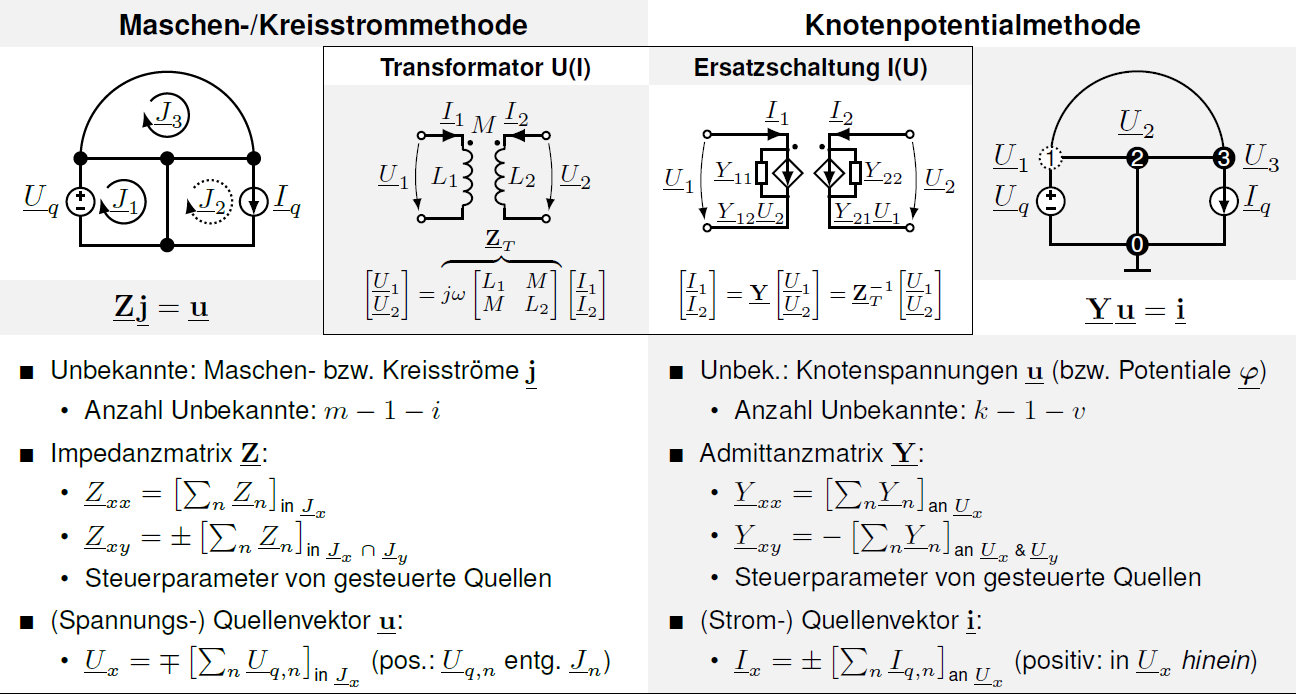
\includegraphics[width=18cm]{maschen.png}\\
		\end{tabular}\\
		
		\hline
	\end{tabular}
		\begin{tabular}{ | c   p{18cm} |}
		\hline
		\cellcolor{black}\rotcell{\large\textbf{\textcolor{white}{Schwingkreise}}}  &
		\setlength{\extrarowheight}{10pt}	
		
		\begin{tabular}{L{5cm} L{11.8cm}}
			&\\[-20pt]
			
			\rowcolor[rgb]{1,1,1}
			\textbf{Kreisgüte}  \qquad\qquad\qquad Serie-SK: $Q_S$, Parallel-SK:$Q_P$
			&$\displaystyle Q=\frac{1}{B_{\mathrm{rel}}}=\frac{\omega_{m} W}{P} \Rightarrow Q_{S}=\frac{1}{R} \sqrt{\frac{L}{C}}, Q_{P}=\frac{1}{G} \sqrt{\frac{C}{L}}$ \\[5pt]
			
			\rowcolor[rgb]{0.91,0.91,0.91}
			\textbf{Resonanzfrequenz}  \qquad\qquad Eigenfrequenz $\omega_0 = \omega_{r \text{verlustlos}}$
			&$\displaystyle \omega_{r}: \operatorname{Im} Z\left(\omega_{r}\right)=0 \quad$ bzw. $\quad \operatorname{Im} Y\left(\omega_{r}\right)=0$ \\[5pt]
	
			\rowcolor[rgb]{1,1,1}
			\textbf{Extremalfrequenz}  \qquad\qquad Bandbreite$B = \omega_m \pm \omega_{3dB}$
			&$\displaystyle \omega_{m}=\arg \max _{\omega}|Z(\omega)| \quad$ bzw. $\quad \omega_{m}=\arg \max _{\omega}|Y(\omega)|$ \\[5pt]
		
		
		
			\rowcolor[rgb]{0.91,0.91,0.91}
			\textbf{Dämpfungsgrad}  \qquad\qquad Zeitkonstante $\tau$
			&$\displaystyle  \zeta=\frac{1}{2 Q}=\frac{1}{\omega_{0} \tau} \qquad\qquad\qquad [\zeta]=1$ \\[5pt]		
			
			\rowcolor[rgb]{1,1,1}
			\textbf{Natürliche Frequenz}  \qquad\qquad Gedämpfte Eigenfrequenz
			&$\displaystyle \omega_{n}=\omega_{0} \sqrt{1-\zeta^{2}} \qquad\qquad\qquad\left[\omega_{n}\right]=\mathrm{rad} / \mathrm{s}$ \\[5pt]
			
			\rowcolor[rgb]{0.91,0.91,0.91}
			\textbf{Natürliche Schwingung}  \qquad\qquad Freies Ausschwingen 
			&$\displaystyle  a(t)=a_{0} \mathrm{e}^{-t / \tau} \sin \left(\omega_{n} t+\phi\right) \quad a(t)=u(t)$ bzw. $i(t)$ \\[5pt]
			
			
				\rowcolor[rgb]{1,1,1}
			\textbf{Verstimmung}
				 \qquad\qquad normierte(r) Frequenz(gang) 
			&$\displaystyle \nu=\frac{\omega}{\omega_{m}}-\frac{\omega_{m}}{\omega} \qquad\qquad \Omega=\nu Q \qquad\qquad \frac{Z}{R}=1+j \Omega$ \\[5pt]
			
			
			
		\end{tabular}\\
		\hline
	\end{tabular}

	
	%Relativitätstheorie
	\input{sections/relativität.tex}
	
	%Beispiele
	
	%\end{center}

	
	
\end{document}













